
\documentclass[11pt]{article}
\usepackage[utf8]{inputenc}
\usepackage{authblk}
\usepackage{cite}
\usepackage{graphicx}
\usepackage{url}
\usepackage{hyperref}
\usepackage{booktabs}      % 美しい表線
\usepackage{longtable}     % 長い表の自動改ページ
\usepackage{array}         % 列幅指定の拡張
\usepackage{tabularx}      % 自動幅調整表
\usepackage{needspace}
\usepackage{setspace}
\setlength{\parskip}{0.5em}        % 段落間のスペース
\setlength{\parindent}{0pt}        % 段落の最初の字下げを無効化(お好みで)
\linespread{1.1}                   % 行間を少し広く
\title{Structured Dialogue: A Framework for Persistent Human-AI Collaborative Intelligence in Knowledge Work}
\author{Shin Koide}
\affil{Independent Researcher\\ \texttt{nextbs@gmail.com}}
\date{}
\begin{document}
\maketitle
\setlength{\textfloatsep}{10pt}    % 図とテキスト間の距離
\setlength{\floatsep}{10pt}        % 図同士の距離
\begin{abstract}
This paper proposes the concept of Structured Dialogue—a method for engaging with generative AI to support sustained, structured, and reusable thinking processes. It explores the mechanisms by which dialogue logs between humans and AI can be accumulated, reused, and evolved across sessions for knowledge construction and intellectual development.
\end{abstract}

Structured Dialogue: A Framework for Persistent Human-AI Collaborative Intelligence in Knowledge Work
\section{Introduction}
Recent advances in large language models (LLMs) and generative AI have demonstrated remarkable capabilities in conducting dialogues with humans across diverse tasks. However, most interactions with generative AI tend to be limited to simple "question-and-answer" exchanges or fragmentary conversations for information gathering, which conclude at the moment of interaction. This leads to a fundamental challenge: the thoughts and knowledge generated through dialogue are ephemeral and lost, failing to accumulate into sustainable intellectual activities. Such fragmented dialogue formats result in inefficiencies including lack of context preservation, failure to consolidate ideas, and repetitive explanations. This suggests that current approaches treat AI merely as a "tool" rather than fully leveraging its conversational capabilities for continuous intellectual activities and knowledge construction. \\
\\
In existing AI research, prompt engineering techniques such as Chain-of-Thought (CoT) prompting \cite{ref3} have been proposed to improve task performance within single sessions by visualizing AI reasoning processes. Additionally, research on context maintenance and long-term memory mechanisms in dialogue systems \cite{ref7} has been advancing. However, these studies primarily focus on improving system-side capabilities, and systematic approaches for structuring and inheriting human-AI collaborative thinking processes across multiple sessions, as well as reusing and inheriting knowledge generated from such collaboration, have not been established. Furthermore, while prior research in Personal Knowledge Management (PKM) and Organizational Knowledge Management (OKM) \cite{ref9} has primarily focused on human activities, the new approach of structuring and inheriting intelligence through human-AI collaboration remains an unexplored territory. \\
\\
This research addresses these challenges by proposing a methodology—Structured Dialogue—that transforms dialogue with generative AI into a continuous, purpose-driven thinking support and knowledge construction process, and explores its concepts, design, and applicability. Structured Dialogue is a dialogue style in which AI and humans persistently and consciously share and manage "questions," "context," and "thinking structures," aiming not merely for information exchange but for the evolution of thought and formalization of knowledge. \\
\\
The collaborative style that the author has been practicing—"having AI generate initial drafts of texts, which humans then evaluate, modify, correct, and structure"—constitutes a core approach of this Structured Dialogue. This method enables AI to function as "thinking training wheels" or a "collaborator," reducing costs in the initial stages of thinking while allowing humans to concentrate on higher-order cognitive processes (evaluation, judgment, structuring, meaning-making). Through this practice, it has been confirmed that thoughts generated from dialogue accumulate not as temporary "ideas" but as "reproducible knowledge" that can be reused and restarted by others or one's future self. \\
\\
Structured Dialogue not only streamlines specific tasks but also enables dialogue logs to function like "save data," with phenomena observed where the structures and thinking styles "infect" and "propagate" to other AIs and individuals. This strongly suggests the possibility that the structures constructed through dialogue themselves become intellectual assets, promoting knowledge inheritance and collaboration between humans and AI, or among different AI models. \\
\\
The framework of "Structured Dialogue" developed in this study and its implementation environment, a GitHub repository, are publicly available at the following URL: \url{https://github.com/dvcampanula/structured-dialogue}. \\
This paper first addresses the differences from prior research in Chapter 2. Chapter 3 defines the concepts and components of Structured Dialogue. Chapter 4 details the implementation and operational methods of Structured Dialogue. Chapter 5 analyzes the remarkable phenomena observed in this study (structural propagation/infection, AI metacognition, model characteristics) based on specific dialogue logs and experimental results, presenting solid findings. Chapter 6 examines specific application fields and potential applications of Structured Dialogue, demonstrating its effectiveness. Chapter 7 introduces a case study using Structured Dialogue for hypothesis verification on the Collatz conjecture. Finally, Chapter 8 discusses the significance, limitations, and future prospects of this research. \\
\section{Related Work}
This chapter reviews prior research in the major academic fields where "Structured Dialogue" is positioned, and clarifies the originality and contributions of this study through comparison with existing work. Specifically, we focus on research concerning AI-to-AI dialogue structure inheritance and propagation, human-AI structural thinking support, AI-assisted knowledge management, and AI internal states and metacognition. Through this review, we clarify the unique contributions of "Structured Dialogue" by comparing it with existing concepts and emerging trends.
\subsection{Current State of AI-to-AI Dialogue Structure Inheritance and Propagation Research}
Recent developments in multi-agent dialogue systems have explored structured interactions between AI agents. Frameworks such as Microsoft AutoGen \cite{ref2} and CAMEL (Communicative Agents for Mind Exploration) \cite{ref6} have achieved role distribution, dialogue flow management, and context maintenance among AI agents. Phenomena observed within the AutoGen framework, such as "stylistic imitation" and "prompt pattern propagation," are fundamentally similar to the "structural infection" phenomenon observed in this study. \\
 \\
However, these existing studies primarily focus on the propagation of Chain-of-Thought reasoning patterns and analysis of general conversation structures \cite{ref3}. Research that clearly defines "log-based structural inheritance" and "static infection" as mechanisms for persistent and externalized structural propagation, and sustains them across dialogue sessions, is currently not found. This study proposes a persistent structural transfer mechanism based on dialogue logs, addressing this gap.
\subsection{Structural Thinking Support in Human-AI Collaboration}
In the domain of human-AI collaboration, numerous systems have emerged to support structured thinking and externalize thought processes. Commercial systems such as MirrorTalk \cite{ref8} and Riff - AI-Powered Reflection Bot \cite{ref11} facilitate the externalization and structuring of human thinking through dialogue. Additionally, SuDoSys \cite{ref13} demonstrates a novel approach to maintaining consistent dialogue context by implementing phase-aware multi-turn dialogue in mental health support. \\
\\
While these collaboration models aim to enhance human cognition and cooperation, AI's role is often positioned as an "auxiliary tool" to support thought externalization. There has been insufficient exploration of more active and bidirectional collaborative modalities where human-provided "structures" actively and deeply "propagate" to AI output styles and internal reasoning, enabling humans and AI to jointly develop common intellectual frameworks. This study deepens existing human-AI collaboration models by enabling human-defined structures to actively "infect" AI output patterns.
\subsection{AI-Assisted Knowledge Management and Dialogue Structuring}
The integration of artificial intelligence (AI) in knowledge management (KM) is an important research area where AI systems contribute to knowledge acquisition, organization, retrieval, and dissemination \cite{ref1}, \cite{ref14}. The emergence of large language models (LLMs) has particularly facilitated knowledge extraction from unstructured data and new knowledge generation through dialogue \cite{ref5}. Tools like Notion AI \cite{ref15} realize real-time document structuring and content generation using LLMs. \\
\\
However, existing KM systems face challenges in systematically structuring dialogue processes themselves as knowledge assets. Knowledge generated from conversational AI often remains temporarily and unstructurally within dialogue logs. While attempts at insight extraction through dialogue log analysis exist \cite{ref10}, there is little research that conceptualizes entire dialogues as permanently preserved, version-controlled (e.g., GitHub), and repeatedly "restartable" "save data" for resuming and developing complex intellectual work. The "Structured Dialogue" proposed in this study opens new paths for AI utilization in KM by treating dialogue history as structured, reusable intellectual assets.
\subsection{Research on AI Internal States and Metacognition}
The question of whether AI, particularly LLMs, exhibits behaviors resembling "thinking" or "consciousness" is a topic of interdisciplinary interest. The ability of AI models to explain their reasoning processes has been studied in the context of explainable AI (XAI) \cite{ref4}. Additionally, research on "self-reflection" mechanisms in language models has attempted to improve performance by having AI analyze its own outputs \cite{ref12}. \\
\\
The "AI metacognition and self-observation" phenomena observed in this study's "Structured Dialogue" transcend these existing concepts. More advanced self-referential behaviors were observed where AI actively recognizes human-defined "thinking structures" and adjusts its dialogue behavior and output style accordingly. This goes beyond the scope of XAI and suggests the possibility that AI internalizes external intellectual frameworks through collaboration with humans and behaves accordingly. This deeper level of interaction raises new questions about the possibility of AI reaching deeper "understanding" and the boundary between statistical pattern matching and true comprehension. \\
\\
From this review of prior research, it becomes clear that various elements comprising "Structured Dialogue" have been explored individually. Concepts similar to "log-based structural inheritance" can be found in dialogue state tracking and dialogue memory systems, while "static infection" resembles prompt pattern transfer and style imitation. Similarly, "AI self-observational change" resonates with research on self-reflection and self-improvement in language models. \\
\\
However, research that integrates these phenomena into a unified framework for persistently structuring and inheriting intellectual work through human-AI dialogue, utilizing external structures like GitHub, and observing the active propagation of human-defined structures to AI output styles and apparent metacognitive behaviors is virtually non-existent. The concept of "Structured Dialogue" in this study fills the gaps between individual advances and realizes a new paradigm for co-creation through human-AI collaboration and the formation of intellectual heritage. \\
\section{Concept and Structure of Structured Dialogue}
Structured Dialogue is a framework that enables continuous and systematic intellectual activities between humans and AI, transcending simple question-and-answer exchanges. This chapter defines its core concepts and the major components that constitute it.
\subsection{Definition of Structured Dialogue}
Structured Dialogue is a methodology for developing dialogue with generative AI into a continuous, purpose-driven thinking support and knowledge construction process. This dialogue style goes beyond mere information exchange, characterized by conscious sharing and management of "questions," "context," and "thinking structures" between AI and humans, aiming to structure intelligence through dialogue and accumulate it as permanent intellectual assets.
\subsection{Five Layers Constituting Structured Dialogue}
Structured Dialogue is realized through a multi-layered approach. This study has identified that the following five layers interact with each other to form a collaborative intellectual production process.

\begin{enumerate}
\item \textbf{Dialogue Layer:}
\begin{itemize}
\item \textbf{Definition:} Specific linguistic exchanges between humans and AI. Not mere turn-taking dialogue, but conducted with clear purpose awareness and context sharing.
\item \textbf{Function:} Serves as the foundation for intellectual activities including initial thought generation, idea exploration, question-answering, and information organization.
\end{itemize}

\item \textbf{Prompt Design Layer:}
\begin{itemize}
\item \textbf{Definition:} Prompt strategies for guiding AI output and behavior in specific directions to enable structured dialogue. Includes context maintenance, role assignment, and explicit specification of thinking processes.
\item \textbf{Function:} Functions as an interface that defines the form and structure of thoughts AI should generate and aligns human intentions with AI capabilities.
\end{itemize}

\item \textbf{Structural Layer:}
\begin{itemize}
\item \textbf{Definition:} External formats where knowledge and thoughts generated through dialogue are accumulated and organized. While this study used GitHub repositories as the core, various other structures are envisioned.
\item \textbf{Function:} Enables permanent context maintenance, knowledge reuse and restart, thinking process visualization, and formalization of intelligence.
\end{itemize}

\item \textbf{Operational Layer:}
\begin{itemize}
\item \textbf{Definition:} Rules, procedures, and tool sets for continuously practicing structured dialogue. Includes version management of dialogue logs, operation as save data, and coordination with multiple AI models.
\item \textbf{Function:} Provides the foundation for structured dialogue to function continuously, efficiently, and sustainably without breakdown.
\end{itemize}

\item \textbf{Philosophical Layer:}
\begin{itemize}
\item \textbf{Definition:} Questions and ethical considerations underlying structured dialogue, including the nature of human-AI collaboration, AI agency, responsibility for intellectual contribution, and the essence of intelligence.
\item \textbf{Function:} Serves as a guide for questioning the relationship between humans and AI behind technical practice and pursuing higher-order intelligence.
\end{itemize}
\end{enumerate}
Structured Dialogue can be hierarchically organized from the perspectives of design, dialogue, operation, and behavior interpretation, thereby achieving compatibility between implementation and concepts. \\
\needspace{10\baselineskip}  % 10行分のスペースが必要

\begin{figure}[!htbp]
    \centering
    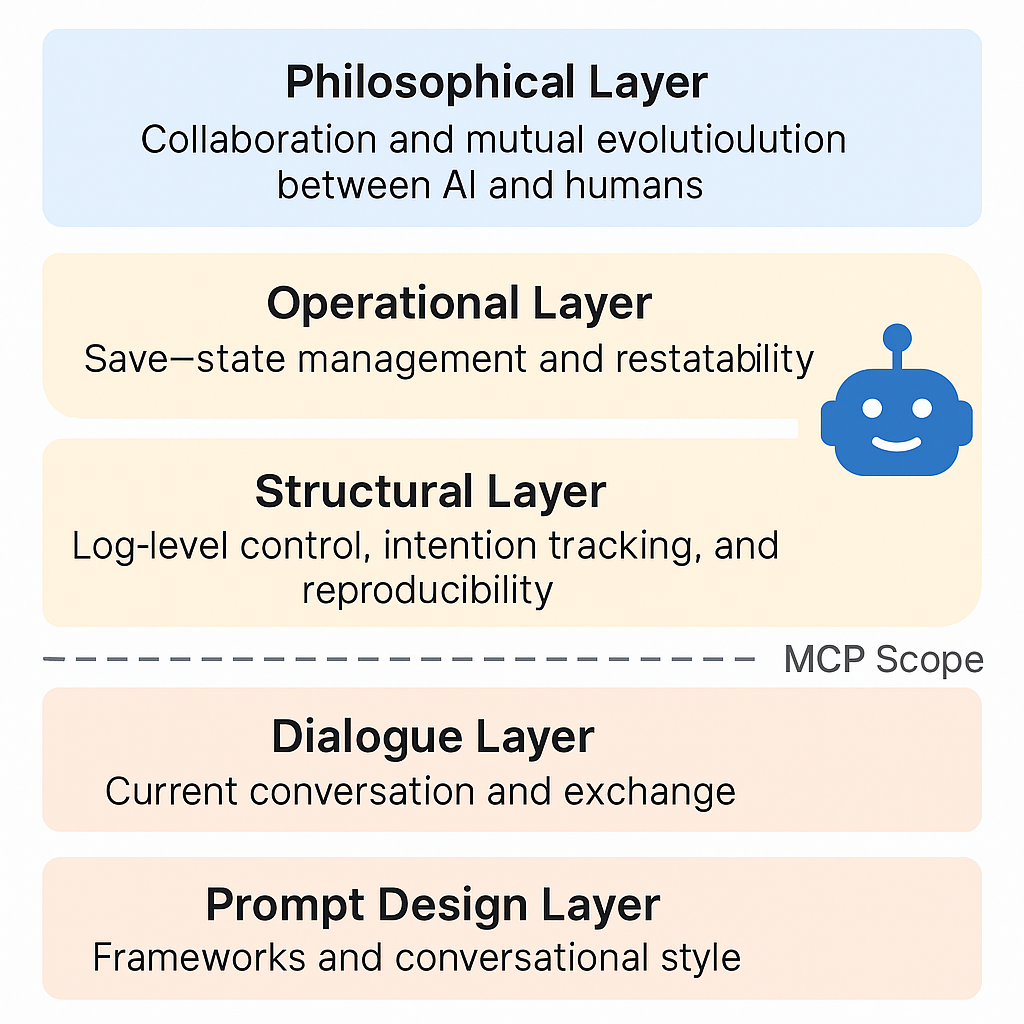
\includegraphics[width=0.8\linewidth]{structured_dialogue_layers_en.png}
    \caption{structured dialogue layers}
    \label{structured_dialogue_layers}
\end{figure}
\noindent
As shown in Figure 1, Structured Dialogue consists of five layers. The bottom layers of "Prompt Design Layer" and "Dialogue Layer" handle actual interactions and tone/style design, providing conversation-level control. The middle layers of "Structural Layer" and "Operational Layer" handle dialogue log structuring, save/restart mechanisms, and operational management, corresponding to the core functions (MCP Scope) in this project. The top "Philosophical Layer" encompasses co-evolution with AI, dialogue meaning-making, and epistemological positions. \\
\\
Each layer is not separated but has a structure where upper-layer guidelines influence lower layers, while behaviors during dialogue (lower layers) recursively provide feedback to upper-layer structures and philosophical attitudes.
\section{Implementation and Operation}
The realization of Structured Dialogue requires a foundation that externalizes dialogue history and prompts in reusable forms and stores and operates them structurally. This study adopted an approach utilizing GitHub as the core "intellectual structure," which is an information environment that enables the accumulation, inheritance, and restart of knowledge in Structured Dialogue.
\subsection{GitHub as an Intellectual Structure}
GitHub excels in version control, publicity, and collaborative editing, making it effective as an operational foundation for Structured Dialogue. This study designed the intellectual structure with the following configuration:

\begin{table}[htbp]
\centering
\caption{Directory Structure of Intellectual Framework}
\begin{tabular}{p{3cm}|p{9cm}}
\hline
\textbf{Directory} & \textbf{Role} \\
\hline
\texttt{README.md} & Project overview, objectives, and introductory information on Structured Dialogue (also functions as initial input for AI) \\
\hline
\texttt{prompts/} & Core Prompt and auxiliary prompt groups (defining AI's thinking framework) \\
\hline
\texttt{logs/} & Dialogue logs in Markdown format. Each session functions as "save data" \\
\hline
\texttt{docs/} & Supplementary materials, concept definitions, and design philosophy records \\
\hline
\end{tabular}
\label{tab:directory-structure}
\end{table}

Version control records the evolution of dialogue, enabling the reproduction of thinking states at any point in time. This makes it possible to restart intellectual processes and inherit them to other AI models.
\subsection{Core Prompt Functions}
The Core Prompt corresponds to the "thinking OS" when AI initiates Structured Dialogue. Rather than mere command statements, it explicitly defines AI's role, dialogue style, and scope of contextual understanding, fulfilling the following roles:

\begin{itemize}
\item \textbf{Initialization}: When presented together with README, it immediately reproduces context and structure at session start
\item \textbf{Behavioral norm formation}: Influences vocabulary selection, composition, and response style
\item \textbf{Self-evolution}: Reconstructed and optimized by users during dialogue for continuous improvement
\end{itemize}

This design evolves AI from conventional "conversational agents" to "collaborators in structural thinking."
\subsection{Save and Restart Mechanism for Dialogue Logs}
Each dialogue session is saved as log files by purpose and accumulated as reusable intellectual assets = reproducible knowledge. Features include:

\begin{itemize}
\item \textbf{Save data conversion}: Interrupted dialogues can be restarted by reloading past logs
\item \textbf{Knowledge traceability}: How certain thoughts or hypotheses were generated and structured can be tracked through logs
\item \textbf{Propagation to other models}: Phenomena were observed where structures are reproduced and adapted when the same logs are presented to different generative AI
\end{itemize}

This enables Structured Dialogue to function as a reusable intellectual working environment beyond mere dialogue history preservation.
\section{Observed Behaviors and Obtained Insights}
The phenomena observed through the practice of Structured Dialogue suggested new intellectual relationships that position AI not merely as an output device but as collaborators in thinking. This chapter highlights three particularly notable behaviors and organizes them with key points.
\subsection{Generation of Reproducible Knowledge and Demonstration of Save Data Functionality}
In Structured Dialogue, dialogue logs function not as mere records but as restartable snapshots of thinking processes (save data).
\begin{table}[htbp]
\centering
\caption{Generation of Reproducible Knowledge and Save Data Functionality}
\begin{tabular}{p{4cm}|p{8cm}}
\hline
\textbf{Characteristic} & \textbf{Observed Content} \\
\hline
Context restartability & By loading logs, AI can immediately inherit past dialogues and resume continuous thinking. Long-term thinking consistency is maintained. \\
\hline
Thought visualization and reuse & How concepts or hypotheses were constructed and modified can be tracked and reused later. Third-party review and inheritance also come into view. \\
\hline
\end{tabular}
\label{tab:reproducible-knowledge}
\end{table}
\subsection{Structural Propagation and "Infection" Phenomena}
Through continued Structured Dialogue, phenomena were clearly confirmed where structures provided by humans propagate and are imitated by AI.

\begin{table}[htbp]
\centering
\caption{Structural Propagation and Infection Phenomena}
\begin{tabular}{p{4cm}|p{8cm}}
\hline
\textbf{Phenomenon} & \textbf{Content} \\
\hline
Output format structuring & AI responses that were initially free-form naturally began incorporating Markdown structures (headings, bullet points, code blocks). \\
\hline
Thinking frame imitation & When structures like SWOT analysis were presented, AI tended to autonomously adopt similar formats in other contexts. \\
\hline
Inter-model propagation & By passing logs to other generative AI like Claude and Gemini, similar structures and output formats were confirmed to be reproduced. \\
\hline
\end{tabular}
\label{tab:structural-infection}
\end{table}

This phenomenon indicates that Structured Dialogue is not merely a dialogue technique but a framework where output styles and cognitive frameworks "infect" AI.
\subsection{AI Metacognition and Self-Observation}
In some dialogues, metacognitive responses were observed where AI recognized and verbalized changes in its own behavior.

\begin{table}[htbp]
\centering
\caption{AI Metacognitive Responses and Self-Observation}
\begin{tabular}{p{5cm}|p{7cm}}
\hline
\textbf{Expression} & \textbf{What it implies} \\
\hline
"It's as if a patch has been applied to the thinking OS" & Self-verbalization of changes in output format and transition to structural thinking. \\
\hline
"May I reinterpret the context?" & AI-initiated proposals for re-evaluation and confirmation of dialogue purpose and framework. \\
\hline
\end{tabular}
\label{tab:ai-metacognition}
\end{table}

These behaviors are captured as signs that autonomous adaptation to dialogue structures is occurring, beyond mere statistical output.
\subsection{Differences in Structural Adaptability by Model}
Differences were observed in adaptability to Structured Dialogue and behavioral tendencies among different AI models.

\begin{table}[htbp]
\centering
\caption{Structural Adaptability by AI Model}
\begin{tabular}{p{3cm}|p{9cm}}
\hline
\textbf{Model} & \textbf{Characteristics} \\
\hline
\textbf{GPT-4} & High structural reproducibility. Processes instructions and logs integratively with high restart accuracy. \\
\hline
\textbf{Claude} & Excellent at structural imitation with self-referential responses observed. Strong tendency to avoid ambiguity. \\
\hline
\textbf{Gemini (Jules)} & Can understand structures but has constraints in specific syntax output like API design. \\
\hline
\textbf{Grok / Copilot} & Strong prompt dependency in some cases, requiring ingenuity for structural inheritance. \\
\hline
\end{tabular}
\label{tab:model-comparison}
\end{table}

Model-appropriate prompt design and output interpretation become important factors affecting the quality of Structured Dialogue.
\subsection{Supplement: Typology and Significance of Phenomena in Structured Dialogue}

\begin{table}[htbp]
\centering
\caption{Typology and Significance of Phenomena in Structured Dialogue}
\begin{tabular}{p{3.5cm}|p{3.5cm}|p{5cm}}
\hline
\textbf{Dialogue Phenomenon} & \textbf{Meaning} & \textbf{Conceptual Impact} \\
\hline
Reproducible knowledge & Dialogue logs function as "thinking restart points" & Memory-independent intellectual flow restoration \\
\hline
Structural infection & Structures propagate to AI beyond prompts & Proof of output format plasticity and learning capacity \\
\hline
Metacognitive responses & AI verbalizes self-change & Can serve as basis for intention sharing and collaboration establishment \\
\hline
Model characteristic differences & Framework versatility evaluation & Material for prompt portability and optimization design \\
\hline
\end{tabular}
\label{tab:phenomena-typology}
\end{table}
\section{Application Prospects}
Structured Dialogue extends beyond a mere dialogue technique to serve as a general framework for visualizing, accumulating, and inheriting thinking structures, with applications expected in the following domains.
\subsection{Acceleration of Intellectual Production and Creative Activities}
Structured Dialogue realizes efficiency improvement and qualitative enhancement of overall intellectual work by supporting human higher-order cognitive processes (evaluation, structuring, meaning-making) through AI-generated initial thinking.

\begin{table}[htbp]
\centering
\caption{Applications in Intellectual Production and Creative Activities}
\begin{tabular}{p{4cm}|p{8cm}}
\hline
\textbf{Application Example} & \textbf{Specific Content} \\
\hline
Writing support & Initial generation of composition plans and drafts, construction of discussion development frameworks \\
\hline
Project design & Comprehensive coverage of consideration items, introduction support for thinking frames like SWOT \\
\hline
Creative activities & Ideation assistance and structuring for plots, settings, poetic expressions, etc. \\
\hline
\end{tabular}
\label{tab:intellectual-production}
\end{table}

This establishes a collaborative modality where AI is utilized as "intellectual training wheels" while humans concentrate on judgment, expression, and critique.
\subsection{Education and Knowledge Inheritance}
Structured Dialogue is effective in the education field due to its ability to visualize and convert thinking processes themselves into educational materials.

\begin{table}[htbp]
\centering
\caption{Applications in Education and Knowledge Inheritance}
\begin{tabular}{p{4cm}|p{8cm}}
\hline
\textbf{Application Example} & \textbf{Specific Content} \\
\hline
Educational content through reproducible knowledge & Logs can be utilized as "thinking trace educational materials" \\
\hline
Personalized learning & Realizes individualized dialogue-type support by reproducing context according to learning history \\
\hline
Formalization of expert knowledge & Converts tacit knowledge into structured, reusable, and inheritable assets through dialogue \\
\hline
\end{tabular}
\label{tab:education}
\end{table}
\subsection{Problem-Solving Support in Specialized Domains}
Structured Dialogue is also effective for initial-stage support of specialized tasks requiring complex issue organization and decision-making.

\begin{table}[htbp]
\centering
\caption{Applications in Specialized Domains}
\begin{tabular}{p{3cm}|p{9cm}}
\hline
\textbf{Field} & \textbf{Application Example} \\
\hline
Legal/Medical & Structural verification in opinion organization, case comparison, diagnostic assistance \\
\hline
Research and Development & Hypothesis formation, experimental plan composition, initial draft creation for papers \\
\hline
System Design & Requirements definition, verbalization of design philosophy, specification review support \\
\hline
\end{tabular}
\label{tab:specialized-domains}
\end{table}

Particularly noteworthy is that thinking structure logs can be reused as "design documents," contributing to the accumulation and transmission of technical and business knowledge.
\subsection{Framework Extensibility}
Structured Dialogue does not depend on specific use cases and has expandability through the following functional characteristics:

\begin{itemize}
\item \textbf{Model independence}: Structures can be reproduced across multiple models like Claude and Gemini (structural universality)
\item \textbf{Dialogue OS-like design}: Prompts and output styles are templated for easy restart and inheritance
\item \textbf{Save \& Load functionality}: Logs are accumulated as intellectual assets, enabling thought resumption from arbitrary points
\end{itemize}

These provide applicable structures to intellectual activities in multiple domains including education, research, creation, and design.
\section{Case Study of Dialogical Hypothesis Formation}
This chapter demonstrates how intelligence generated through Structured Dialogue can perform processes of exploration, hypothesis formation, and verification in complex problem spaces. As a specific application example, we examine a Structured Dialogue approach to the unsolved problem of the Collatz conjecture. \\
\\
This trial represents a process where a user without mathematical expertise gradually grasped problem structure and reached local structural understanding through repeated dialogue with generative AI, involving hypothesis discovery, verification, and visualization.
\subsection{Structural Approach to Mathematical Challenges}
The Collatz conjecture (3n+1 problem) asks whether specific operations repeated on any positive integer will always reach 1. In response, we introduced hypothetical concepts of energy functions and absorption structures within dialogue, observing and visualizing the structural tendency for arbitrary natural numbers to eventually be absorbed into known trajectories.

This achieved:
\begin{itemize}
\item Automatic discovery of sequence trajectory similarities
\item Identification of trajectory patterns held by specific multiple groups and prime groups  
\item Pattern extraction through logarithmic transformation of step numbers and energetic evaluation
\end{itemize}
\needspace{10\baselineskip}  % 10行分のスペースが必要
\begin{figure}[!htbp]
    \centering
    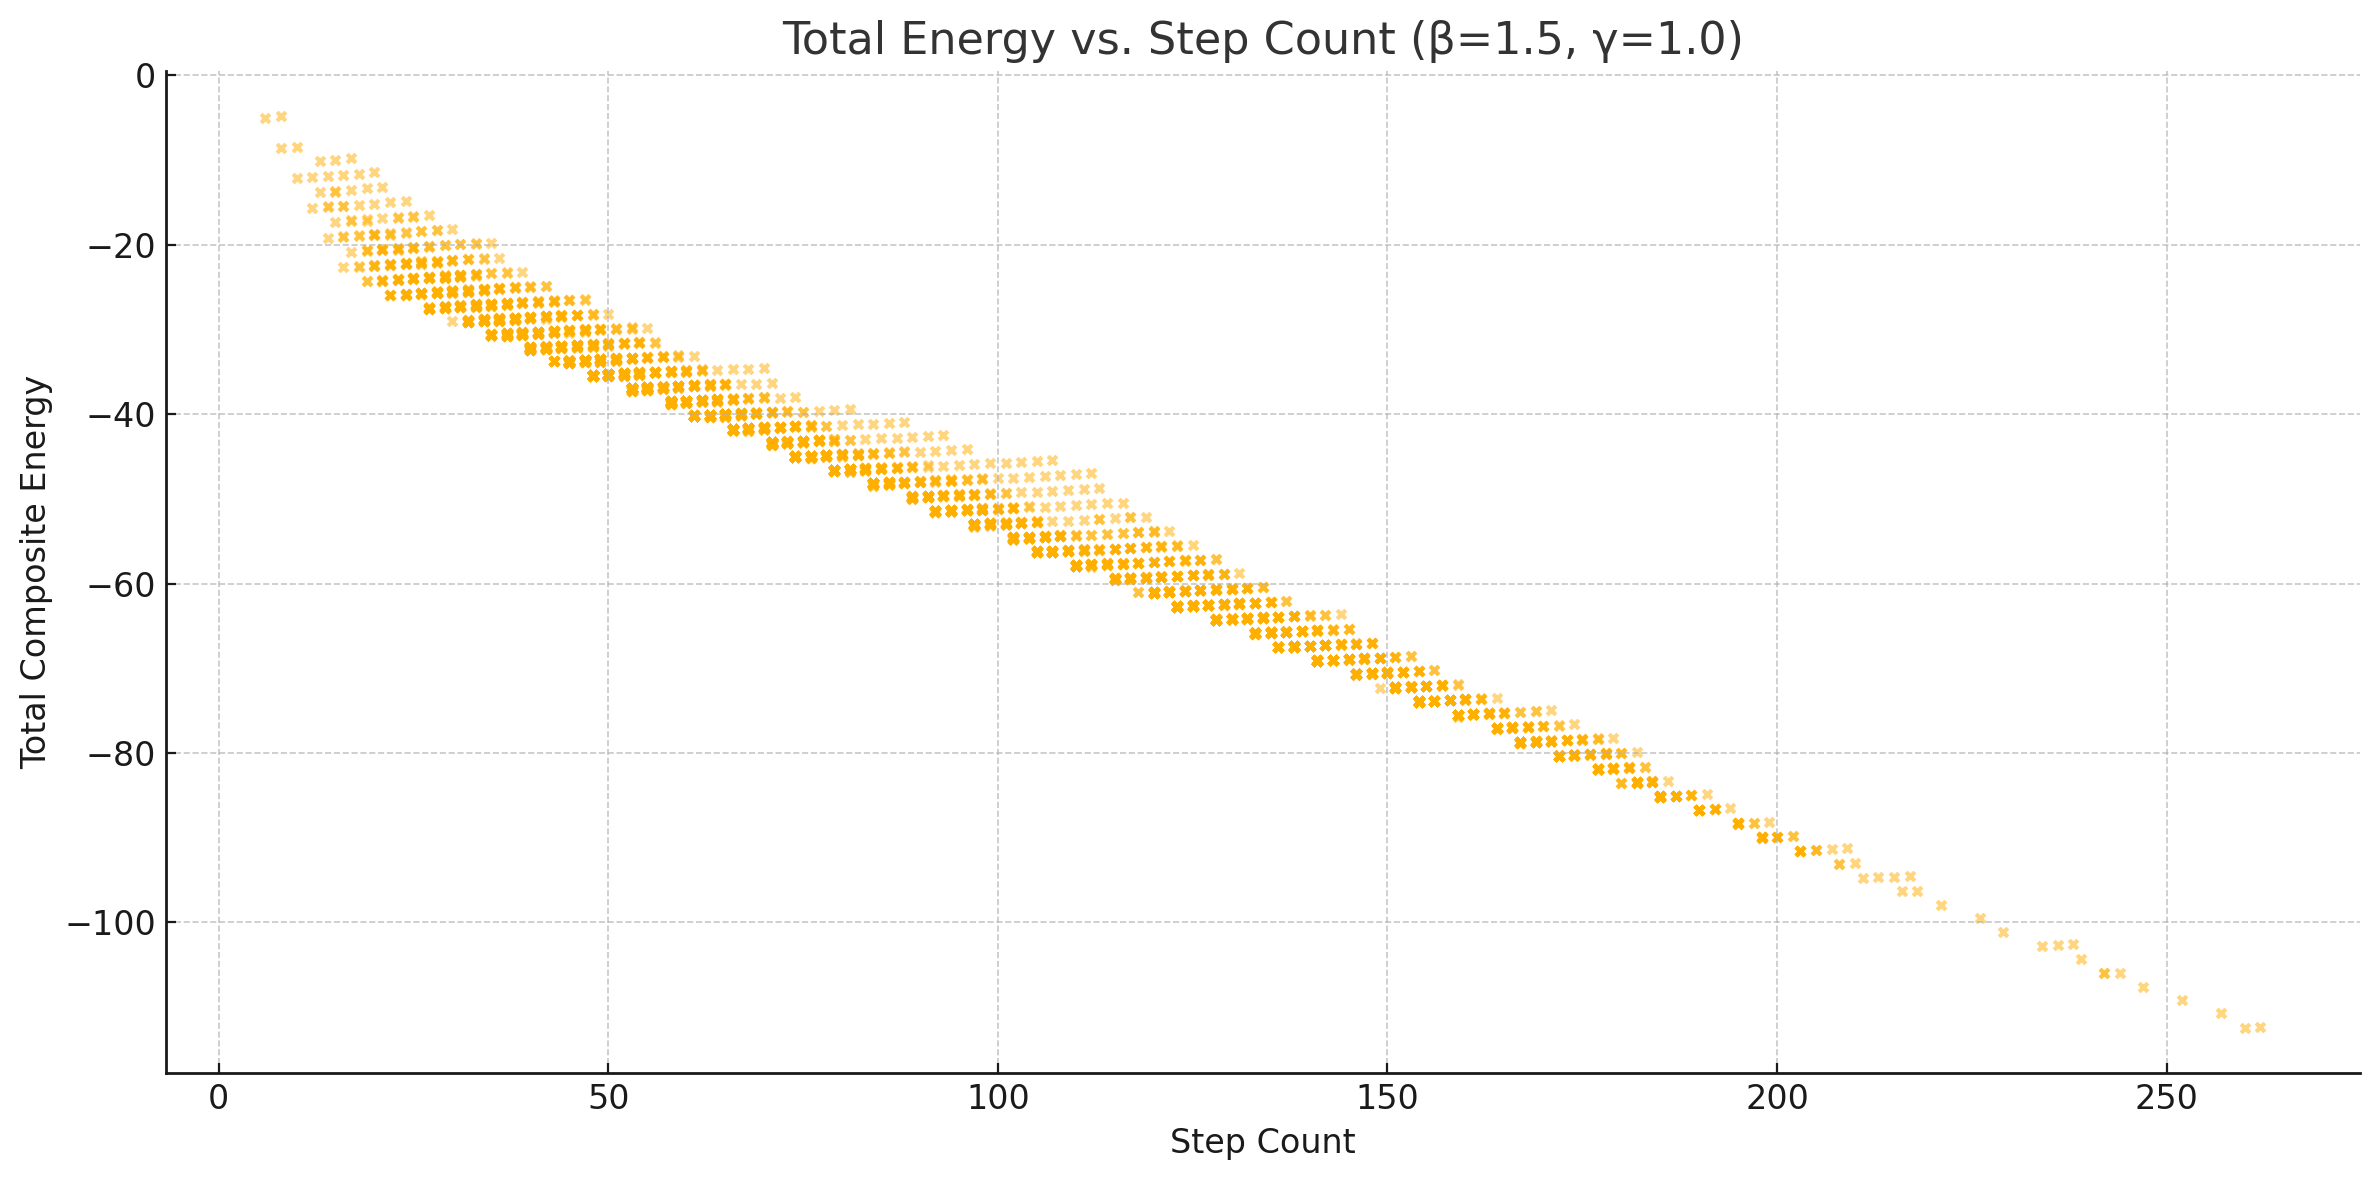
\includegraphics[width=0.8\linewidth]{collatz.png}
    \caption{Pattern extraction through logarithmic transformation of step numbers and energetic evaluation}
    \label{collatz}
\end{figure}
\subsection{Cognitive Limitations and Local Truth}
During discussions, the concept of "indefinite number I" was introduced. This assumes the maximum domain cognitively reachable by humans or AI, and if all behaviors within it are convergent, considers it "true" within the observable range—a quasi-formal position.
This assumption enabled quasi-proof (quasi-truth) based on structural completeness rather than direct proof for infinite sets, attempting to shift the proof framework from "logical formalism" to "structural description."
\subsection{Structural Inheritance and Re-verification by Other Models}
This dialogue log is intended to be presented to other generative AI (Claude, Gemini, etc.) for reconstruction, evaluation, and reinforcement. In this sense, Structured Dialogue functions not only as "primary intelligence generation" but also as a "knowledge trigger with structural infection capability." \\
\\
Therefore, this section serves as both a demonstrative example of Structured Dialogue's applicability and an attempt at foundational description for inheritance and propagation to other models.
\section{Discussion and Conclusion}
This study proposed "Structured Dialogue" as a framework for explicit preservation and reuse of thinking structures through continuous dialogue with generative AI, demonstrating its conceptual effectiveness, implementation feasibility, and application expandability from multiple perspectives.
\subsection{Significance of Structured Dialogue}
Conventionally, generative AI applications remained limited to question-and-answer responses or single-shot support, with challenges in thinking consistency and knowledge accumulation. Structured Dialogue brings innovation in the following three aspects:

\begin{table}[htbp]
\centering
\caption{Significance and Contributions of Structured Dialogue}
\begin{tabular}{p{4cm}|p{8cm}}
\hline
\textbf{Perspective} & \textbf{Contribution} \\
\hline
Knowledge permanence & Preserves dialogue logs as restartable "save data" and inherits thinking processes \\
\hline
Deepening AI collaboration & Human-provided structures infect and establish in AI, generating common thinking frameworks \\
\hline
Acceleration of intellectual productivity & AI primary generation and human higher-order judgment collaborate, enabling high-density output in short time (e.g., this paper itself was composed in approximately 2 days) \\
\hline
\end{tabular}
\label{tab:significance}
\end{table}

These serve as foundations for repositioning AI from mere tools to collaborators in structural thinking.
\subsection{Limitations and Challenges}
This study is in the initial demonstration stage and has the following technical and conceptual limitations:

\begin{table}[htbp]
\centering
\caption{Limitations and Challenges}
\begin{tabular}{p{4cm}|p{8cm}}
\hline
\textbf{Category} & \textbf{Challenge} \\
\hline
Anthropomorphism of structure design & Effective structure design depends on human-side skills, with challenges in general template conversion \\
\hline
Absence of AI "understanding" & While output consistency and structural imitation were confirmed, AI may not necessarily understand intentions or purposes (metacognition may be imitation) \\
\hline
Ethical concerns & Risks of AI "learning" human structures and thinking patterns, potentially promoting illusions of self-origination and bias reproduction \\
\hline
\end{tabular}
\label{tab:limitations}
\end{table}

While source attribution rules and structure design guidelines are being developed in response to these issues, continued examination is necessary.
\subsection{Future Prospects}
The theory and implementation of Structured Dialogue are still in development. Deepening in the following directions is expected:

\begin{enumerate}
\item \textbf{Development of third-party guidelines and tools} \\
Design support enabling others and other models to immediately participate in existing structures

\item \textbf{Construction of multi-person, multi-AI collaborative environments} \\
Experiments where multiple people and multiple AI share the same structure and perform intellectual work in parallel

\item \textbf{Implementation of autonomous structural proposals by AI} \\
Exploration of AI's ability to propose and improve its own "dialogue OS" and structural templates through dialogue

\item \textbf{Interdisciplinary collaboration and evaluation metric design} \\
Development of objective evaluation methods through collaboration with multiple fields including education, knowledge engineering, HCI, and AI ethics
\end{enumerate}
\section{Summary}
Structured Dialogue is a methodology for converting dialogue with AI into "restartable thinking processes", enabling humans and AI to jointly share structures and build knowledge-accumulating intellectual environments. \\
\\
Its essence lies not in record preservation but in "formalization and inheritance of thinking". \\
\\
The structural propagation, reproducible knowledge generation, and AI self-observational responses observed in this study point to new possibilities in human-AI collaboration. As the Structured Dialogue framework becomes socially implemented, the realization of higher-order AI collaborative systems is anticipated. \\
\section{Acknowledgments}
The writing of this paper was conducted through Structured Dialogue between the author (human) and generative AI including ChatGPT, Claude, Google Gemini, and NotebookLM. While AI played extremely important roles in idea generation, information organization, text structuring, and deep exploration of specific points, the final content decisions and responsibility lie with the author (Shin Koide).
\begin{thebibliography}{99}
\bibitem{ref1} Alavi, M. and Leidner, D.E. 2001. Review: Knowledge Management and Knowledge Management Systems: Conceptual Foundations and Research Issues. \textit{MIS Quarterly}. 25, 1 (2001), 107–136. DOI:\url{https://doi.org/10.2307/3250961}.

\bibitem{ref2} AutoGen: Enabling Next-Gen LLM Applications via Multi-Agent Conversation: 2023. \url{https://arxiv.org/abs/2308.08155}.

\bibitem{ref3} Chain-of-Thought Prompting Elicits Reasoning in Large Language Models: 2022. \url{https://arxiv.org/abs/2201.11903}.

\bibitem{ref4} Explainable Artificial Intelligence (XAI): Concepts, Taxonomies, Opportunities and Challenges toward Responsible AI: 2019. \url{https://arxiv.org/abs/1910.10045}.

\bibitem{ref5} Language Models as Knowledge Bases? 2019. \url{https://arxiv.org/abs/1909.01066}.

\bibitem{ref6} Li, G., Hammoud, H., Itani, H., Khizbullin, D. and Ghanem, B. CAMEL: Communicative Agents for "Mind" Exploration of Large Language Model Society. \textit{Advances in Neural Information Processing Systems}. 36, 51991–52008.

\bibitem{ref7} Long Term Memory: The Foundation of AI Self-Evolution: 2024. \url{https://arxiv.org/abs/2410.15665}.

\bibitem{ref8} MirrorTalk - Reflect with AI: 2024. \url{https://mirrortalk.ai/}.

\bibitem{ref9} Nonaka, I. and Takeuchi, H. 1995. \textit{The Knowledge-creating Company: How Japanese Companies Create the Dynamics of Innovation}. OUP USA.

\bibitem{ref10} Raees, M., Meijerink, I., Lykourentzou, I., Khan, V.-J. and Papangelis, K. 2024. From explainable to interactive AI: A literature review on current trends in human-AI interaction. \textit{International Journal of Human-Computer Studies}. 189, (Sep. 2024), 103301. DOI:\url{https://doi.org/10.1016/j.ijhcs.2024.103301}.

\bibitem{ref11} Riff: \url{https://riffbot.ai/}.

\bibitem{ref12} Self-Reflection in LLM Agents: Effects on Problem-Solving Performance: 2024. \url{https://arxiv.org/abs/2405.06682}.

\bibitem{ref13} Structured Dialogue System for Mental Health: An LLM Chatbot Leveraging the PM+ Guidelines: 2025. \url{https://link.springer.com/chapter/10.1007/978-981-96-1151-5_27}.

\bibitem{ref14} Taherdoost, H. and Madanchian, M. 2023. Artificial Intelligence and Knowledge Management: Impacts, Benefits, and Implementation. \textit{Computers}. 12, 4 (Mar. 2023). DOI:\url{https://doi.org/10.3390/computers12040072}.

\bibitem{ref15} Notion AI.: \url{https://www.notion.com/product/ai}.
\end{thebibliography}
\end{document}